\chapter{Ausarbeitung}
\section{Aufgabe 1}
\subsection{a}
$n$ ist die Anzahl der Szstemzustandwerte und $m$ ist die Anzahl der Messwerte.\\\\
$\hat{\bm{x}}_{n-1|n-1}$  ($n \times 1$): Der Zustand an $t_{n-1}$, der unter Berücksichtigung auf Beobachtung $\bm{z}_{n-1}$ und prädizierte Zustand $\hat{\bm{x}}_{n-1|n-2}$  wird. \\\\
$\hat{\bm{x}}_{n|n-1}$  ($n \times 1$): Zustand an $t_n$, die von $\bm{x}_{n-1|n-1}$ geschätzt wird. \\\\
$\hat{\bm{x}}_{n|n}$  ($n \times 1$): Der Zustand an $t_{n-1}$, der unter Berücksichtigung auf Beobachtung $\bm{z}_{n}$ und prädizierte Zustand $\hat{\bm{x}}_{n|n-1}$  wird. \\\\
$\bm{\Phi}_n$  ($n \times n$): Übergangsmatrix, die den Zustand an $t_{n-1}$ nach $t_{n}$ schätzt. \\\\
Kovarianzmatrix $\bm{P}_{n-1|n-1}$, $\bm{P}_{n|n-1}$. $\bm{P}_{n|n}$  ($n \times n$):  ähnlich wie Zustandvektor $\hat{\bm{x}}_{n-1|n-1}$, $\hat{\bm{x}}_{n|n-1}$, $\hat{\bm{x}}_{n|n}$.\\\\
$\bm{R}_n$  ($m \times m$): Kovarianzmatrix vom Messrauschen, $\bm{R}_n = E\left(\bm{v}_n \bm{v}_n^T\right)$, $\bm{v}_n$ ist der Messfehler. \\\\
$\bm{K}_n$  ($n \times m$): Kalman Gain ist ein Gewichtsfaktor zur Projektion der Residuen auf die Korrektur des Zustands. \\\\
$\bm{H}_n$  ($m \times n$): Designmatrix beschreibt die Zusammenhang zwischen dem Zustand und Beobachtung. \\\\
$\bm{Q}$  ($n \times n$): Matrix des Prozessrauschens beschreibt die Unsicherheiten aufgrund von Modellierungsfehlern. 
\subsection{b}
Wenn $\bm{P}$ zu gross oder zu klein: keine Einfluss. \\\\
Wenn $\bm{Q}$ zu gross oder $\bm{R}$ zu klein: Die Ergebnisse wird stark von Messwerte beeinflusst, die Kurve ist zickzackartiger. Bei nicht lineare Funktion dauert die Ergebnisse kurze wieder zu richtiger Richtung.\\\\
Wenn $\bm{R}$ zu gross oder $\bm{Q}$ zu klein: Die Kurve ist flache aber es dauert länger wieder zu richtiger Richtung nach Wendung.\\\\
Wenn $\bm{K}$ zu gross: Die Ergebnisse ist abhängiger von die Korrektur, bzw. die Differenz zwischen die Beobachtungen und die geschätzte Zustande. 
\subsection{c}
Solange das Gröenverhältnis zwischen R und Q passt, ist es weitestgehend egal, welche
Genauigkeitsangaben gewählt wurden. 
\subsection{d}
Designmatrix $\bm{H}$, Übergangsmatrix $\bm{\Phi}$, Prozessrauschenmatrix $\bm{Q}$ und Messrauschenmatrix $\bm{R}$ bleiben konstant. $\bm{P}$ und $\bm{K}$ müssen neu berechnet werden. 
\clearpage
\section{Aufgabe 2}
\subsection{Beobachtungen}
Zuerst erstellt man die Beobachtungen, ein Weihnachtsbaum wird mit 131 Punkten gezeichnet:
\begin{figure}[htbp]
	\centering
	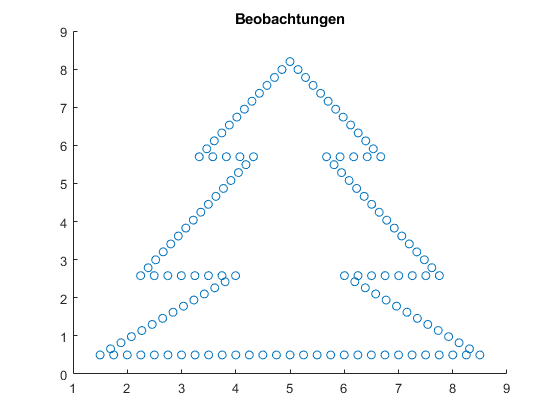
\includegraphics[width=0.9\textwidth]{images/Beobachtung} 
	\caption{Beobachtungen} 
	\label{fig:beobachtung}
\end{figure}
\subsection{KF:Random Walk}
Das Modell von Random Walk:
\begin{gather*}
	\dot{x} = 0 + w(t) \\
	\dot{y} = 0 + w(t)
\end{gather*}
Prozessrauschen und Messrauschen nimmt man bei dieser Aufgabe $\sigma_p = \sigma_r = 0,1$
\begin{gather*}
	\bm{Q} = \begin{bmatrix}
	0,01 & 0 \\
	0 & 0,01
	\end{bmatrix} \\
	\bm{R} = \begin{bmatrix}
	0,01 & 0 \\
	0 & 0,01
	\end{bmatrix}
\end{gather*}
Übergangsmatrix:
\begin{equation*}
	\bm{\Phi} = \begin{bmatrix}
	1 & 0 \\
	0 & 1
	\end{bmatrix}
\end{equation*}
Designmatrix:
\begin{equation*}
	\bm{H} = \begin{bmatrix}
	1 & 0 \\
	0 & 1
	\end{bmatrix}
\end{equation*}
Wir nehmen $y = 5$ und $x = 0.5$ als die Anfangsposition: $\bm{x}_{1|1} = \left[5 \quad  0,5\right]$, $\bm{P}_{1|1} = \begin{bmatrix}
1 & 0 \\
0 & 1
\end{bmatrix}$
\begin{gather*}
	\bm{x}_{n|n-1} = \Phi \cdot \bm{x}_{n-1|n-1} \\
	\bm{P}_{n|n-1} = \Phi \cdot \bm{P}_{n-1|n-1} \\
	\bm{K} = \bm{P}_{n|n-1} \cdot \bm{H}^T \cdot \left(\bm{H} \cdot \bm{P}_{n|n-1} \cdot \bm{H}^T + \bm{R} \right) \\
	\bm{x}_{n|n} = \bm{x}_{n|n-1} + \bm{K} \cdot \left(\bm{z} - \bm{H} \cdot \bm{x}_{n|n-1} \right) \\
	\bm{P}_{n|n} = \left(\bm{I} - \bm{K} \cdot \bm{H}\right) \cdot \bm{P}_{n|n-1}
\end{gather*}
wobei $\bm{z}$ die Beobachtung ist.
\subsection{Integrated Random Walk}
\begin{gather*}
\ddot{x} = 0 + w(t) \\
\ddot{y} = 0 + w(t)
\end{gather*}
Prozessrauschen und Messrauschen nimmt man bei dieser Aufgabe 0,1.
\begin{gather*}
\bm{Q} = \begin{bmatrix}
0,0033 & 0,0050 & 0 & 0 \\
0,0050 & 0,0100 & 0 & 0 \\
0 & 0 & 0,0033 & 0,0050 \\
0 & 0 & 0,0050 & 0,0100 
\end{bmatrix} \\
\bm{R} = \begin{bmatrix}
0,01 & 0 \\
0 & 0,01
\end{bmatrix}
\end{gather*}
Übergangsmatrix:
\begin{equation*}
\bm{\Phi} = \begin{bmatrix}
1 & 1 & 0 & 0 \\
0 & 1 & 0 & 0 \\
0 & 0 & 1 & 1 \\
0 & 0 & 0 & 1
\end{bmatrix}
\end{equation*}
Designmatrix:
\begin{equation*}
\bm{H} = \begin{bmatrix}
1 & 0 & 0 & 0 \\
0 & 0 & 1 & 0 
\end{bmatrix}
\end{equation*}
Die Berechnung danach ist ähnlich wie bei Random Walk.\\\\
Die graphische Darstellung sieht man in \autoref{fig:kleinsigma} \\\\
\begin{figure}[htbp]
	\centering
	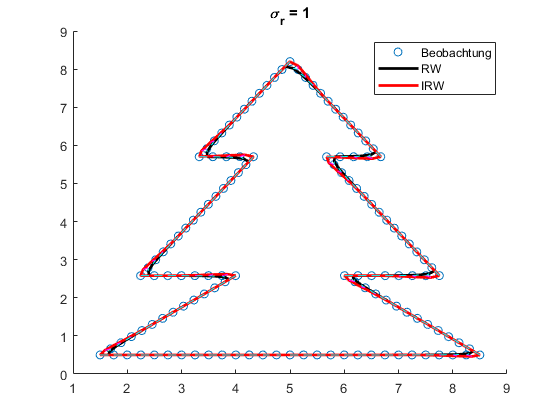
\includegraphics[width=0.65\textwidth]{images/kleinsigma} 
	\caption{$\sigma_r = 0,1$} 
	\label{fig:kleinsigma}
\end{figure}
Die Differenz zwischen die Sollkoordinaten und die Ergebnisse von Kalman Filterung ist in \autoref{fig:diff1}:
\begin{figure}[htbp]
	\centering
	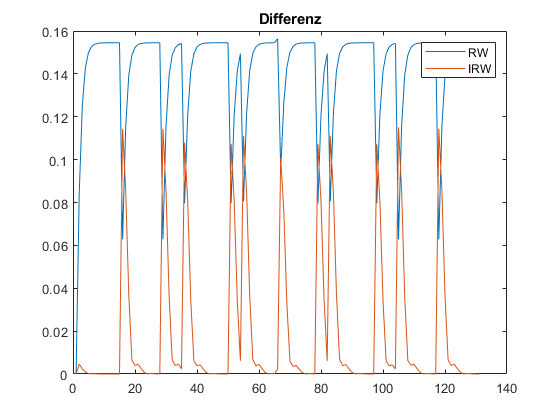
\includegraphics[width=0.55\textwidth]{images/diff1} 
	\caption{Differenzen $\sigma_r = 0,1$} 
	\label{fig:diff1}
\end{figure}\\
\clearpage
Wenn man das Messrauschen $\sigma_r = 1,0$ wählen, wiederholt man das Prozess. Die Ergebnisse sind in \autoref{fig:grosssigma} und die Differenzen sind in \autoref{fig:diff2}. Es ist deutlich zu sehen: die Ergebnisse von Integrated Random Walk sind besser als die von Random Walk. \\\\
Mit größerem Messrauschen weicht das Ergebnis mehr bei den Winkeln ab.
\begin{figure}[htbp]
	\centering
	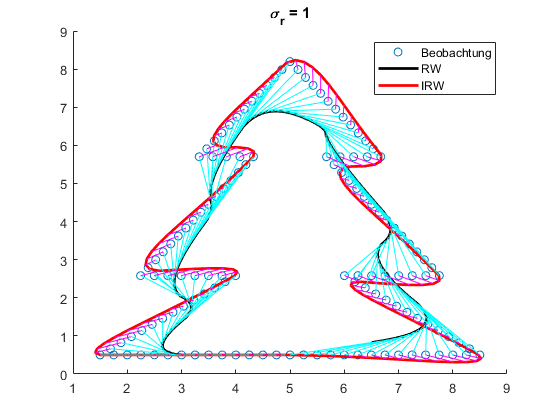
\includegraphics[width=0.55\textwidth]{images/grosssigma} 
	\caption{$\sigma_r = 1$} 
	\label{fig:grosssigma}
\end{figure}
\begin{figure}[htbp]
	\centering
	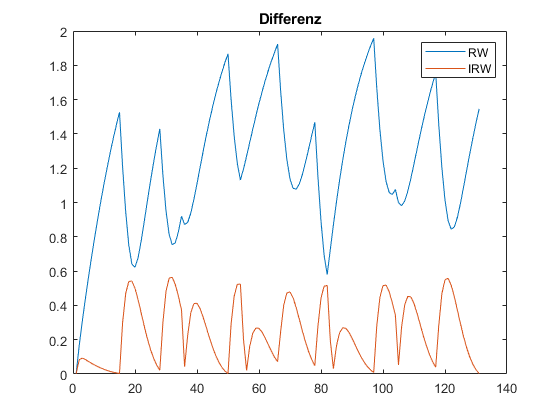
\includegraphics[width=0.65\textwidth]{images/diff2} 
	\caption{Differenzen $\sigma_r = 1$} 
	\label{fig:diff2}
\end{figure}